% Options for packages loaded elsewhere
\PassOptionsToPackage{unicode}{hyperref}
\PassOptionsToPackage{hyphens}{url}
%
\documentclass[
]{article}
\title{Decision Analysis - Bayesian Networks}
\author{Author: Can Aytöre}
\date{Last Update: 2022-02-20}

\usepackage{amsmath,amssymb}
\usepackage{lmodern}
\usepackage{iftex}
\ifPDFTeX
  \usepackage[T1]{fontenc}
  \usepackage[utf8]{inputenc}
  \usepackage{textcomp} % provide euro and other symbols
\else % if luatex or xetex
  \usepackage{unicode-math}
  \defaultfontfeatures{Scale=MatchLowercase}
  \defaultfontfeatures[\rmfamily]{Ligatures=TeX,Scale=1}
\fi
% Use upquote if available, for straight quotes in verbatim environments
\IfFileExists{upquote.sty}{\usepackage{upquote}}{}
\IfFileExists{microtype.sty}{% use microtype if available
  \usepackage[]{microtype}
  \UseMicrotypeSet[protrusion]{basicmath} % disable protrusion for tt fonts
}{}
\makeatletter
\@ifundefined{KOMAClassName}{% if non-KOMA class
  \IfFileExists{parskip.sty}{%
    \usepackage{parskip}
  }{% else
    \setlength{\parindent}{0pt}
    \setlength{\parskip}{6pt plus 2pt minus 1pt}}
}{% if KOMA class
  \KOMAoptions{parskip=half}}
\makeatother
\usepackage{xcolor}
\IfFileExists{xurl.sty}{\usepackage{xurl}}{} % add URL line breaks if available
\IfFileExists{bookmark.sty}{\usepackage{bookmark}}{\usepackage{hyperref}}
\hypersetup{
  pdftitle={Decision Analysis - Bayesian Networks},
  pdfauthor={Author: Can Aytöre},
  hidelinks,
  pdfcreator={LaTeX via pandoc}}
\urlstyle{same} % disable monospaced font for URLs
\usepackage[margin=1in]{geometry}
\usepackage{color}
\usepackage{fancyvrb}
\newcommand{\VerbBar}{|}
\newcommand{\VERB}{\Verb[commandchars=\\\{\}]}
\DefineVerbatimEnvironment{Highlighting}{Verbatim}{commandchars=\\\{\}}
% Add ',fontsize=\small' for more characters per line
\usepackage{framed}
\definecolor{shadecolor}{RGB}{248,248,248}
\newenvironment{Shaded}{\begin{snugshade}}{\end{snugshade}}
\newcommand{\AlertTok}[1]{\textcolor[rgb]{0.94,0.16,0.16}{#1}}
\newcommand{\AnnotationTok}[1]{\textcolor[rgb]{0.56,0.35,0.01}{\textbf{\textit{#1}}}}
\newcommand{\AttributeTok}[1]{\textcolor[rgb]{0.77,0.63,0.00}{#1}}
\newcommand{\BaseNTok}[1]{\textcolor[rgb]{0.00,0.00,0.81}{#1}}
\newcommand{\BuiltInTok}[1]{#1}
\newcommand{\CharTok}[1]{\textcolor[rgb]{0.31,0.60,0.02}{#1}}
\newcommand{\CommentTok}[1]{\textcolor[rgb]{0.56,0.35,0.01}{\textit{#1}}}
\newcommand{\CommentVarTok}[1]{\textcolor[rgb]{0.56,0.35,0.01}{\textbf{\textit{#1}}}}
\newcommand{\ConstantTok}[1]{\textcolor[rgb]{0.00,0.00,0.00}{#1}}
\newcommand{\ControlFlowTok}[1]{\textcolor[rgb]{0.13,0.29,0.53}{\textbf{#1}}}
\newcommand{\DataTypeTok}[1]{\textcolor[rgb]{0.13,0.29,0.53}{#1}}
\newcommand{\DecValTok}[1]{\textcolor[rgb]{0.00,0.00,0.81}{#1}}
\newcommand{\DocumentationTok}[1]{\textcolor[rgb]{0.56,0.35,0.01}{\textbf{\textit{#1}}}}
\newcommand{\ErrorTok}[1]{\textcolor[rgb]{0.64,0.00,0.00}{\textbf{#1}}}
\newcommand{\ExtensionTok}[1]{#1}
\newcommand{\FloatTok}[1]{\textcolor[rgb]{0.00,0.00,0.81}{#1}}
\newcommand{\FunctionTok}[1]{\textcolor[rgb]{0.00,0.00,0.00}{#1}}
\newcommand{\ImportTok}[1]{#1}
\newcommand{\InformationTok}[1]{\textcolor[rgb]{0.56,0.35,0.01}{\textbf{\textit{#1}}}}
\newcommand{\KeywordTok}[1]{\textcolor[rgb]{0.13,0.29,0.53}{\textbf{#1}}}
\newcommand{\NormalTok}[1]{#1}
\newcommand{\OperatorTok}[1]{\textcolor[rgb]{0.81,0.36,0.00}{\textbf{#1}}}
\newcommand{\OtherTok}[1]{\textcolor[rgb]{0.56,0.35,0.01}{#1}}
\newcommand{\PreprocessorTok}[1]{\textcolor[rgb]{0.56,0.35,0.01}{\textit{#1}}}
\newcommand{\RegionMarkerTok}[1]{#1}
\newcommand{\SpecialCharTok}[1]{\textcolor[rgb]{0.00,0.00,0.00}{#1}}
\newcommand{\SpecialStringTok}[1]{\textcolor[rgb]{0.31,0.60,0.02}{#1}}
\newcommand{\StringTok}[1]{\textcolor[rgb]{0.31,0.60,0.02}{#1}}
\newcommand{\VariableTok}[1]{\textcolor[rgb]{0.00,0.00,0.00}{#1}}
\newcommand{\VerbatimStringTok}[1]{\textcolor[rgb]{0.31,0.60,0.02}{#1}}
\newcommand{\WarningTok}[1]{\textcolor[rgb]{0.56,0.35,0.01}{\textbf{\textit{#1}}}}
\usepackage{longtable,booktabs,array}
\usepackage{calc} % for calculating minipage widths
% Correct order of tables after \paragraph or \subparagraph
\usepackage{etoolbox}
\makeatletter
\patchcmd\longtable{\par}{\if@noskipsec\mbox{}\fi\par}{}{}
\makeatother
% Allow footnotes in longtable head/foot
\IfFileExists{footnotehyper.sty}{\usepackage{footnotehyper}}{\usepackage{footnote}}
\makesavenoteenv{longtable}
\usepackage{graphicx}
\makeatletter
\def\maxwidth{\ifdim\Gin@nat@width>\linewidth\linewidth\else\Gin@nat@width\fi}
\def\maxheight{\ifdim\Gin@nat@height>\textheight\textheight\else\Gin@nat@height\fi}
\makeatother
% Scale images if necessary, so that they will not overflow the page
% margins by default, and it is still possible to overwrite the defaults
% using explicit options in \includegraphics[width, height, ...]{}
\setkeys{Gin}{width=\maxwidth,height=\maxheight,keepaspectratio}
% Set default figure placement to htbp
\makeatletter
\def\fps@figure{htbp}
\makeatother
\setlength{\emergencystretch}{3em} % prevent overfull lines
\providecommand{\tightlist}{%
  \setlength{\itemsep}{0pt}\setlength{\parskip}{0pt}}
\setcounter{secnumdepth}{5}
\ifLuaTeX
  \usepackage{selnolig}  % disable illegal ligatures
\fi
\usepackage[]{natbib}
\bibliographystyle{plainnat}

\begin{document}
\maketitle

{
\setcounter{tocdepth}{2}
\tableofcontents
}
\hypertarget{introduction}{%
\section{Introduction}\label{introduction}}

\hypertarget{aim}{%
\subsection{Aim}\label{aim}}

\hypertarget{motivation}{%
\subsection{Motivation}\label{motivation}}

\begin{itemize}
\tightlist
\item
  We have an understanding of BNs as graphical models representing probability distributions.
\item
  What does that imply in terms of the underlying probability distribution?
\item
  What happens if a probability distribution factorizes with respect to a graph?
\item
  What kind of computations can we make on BNs?
\item
  What kind of questions can we answer using (quantified) BNs?
\end{itemize}

\hypertarget{getting-started-with}{%
\section{Getting Started with \ldots{}}\label{getting-started-with}}

\hypertarget{what-is-bn}{%
\subsection{What is BN?}\label{what-is-bn}}

A Probabilistic Network (aka causal graph, Bayesian belief network, etc.) is a graphical representation of a \textbf{joint probability distribution}.

\hypertarget{running-example-is-the-family-out}{%
\subsection{Running Example: ``Is the Family Out?''}\label{running-example-is-the-family-out}}

When Mr.~West goes home at night, he wants to know if his family is home before trying the doors (maybe because the most convenient door to enter is double locked when nobody is home.) Often, when Mrs.~West leaves the house, she turns on an outdoor light. However, she sometimes turns on this light if she is expecting a guest. Also (and of course!) the Wests have a dog. When nobody is home, the dog is put in the backyard. The same is true if the dog has bowel troubles. Finally, if the dog is in the backyard, Mr.~West will probably hear her barking (or what he thinks is her barking), but sometimes he can be confused by other dogs barking.

\begin{Shaded}
\begin{Highlighting}[]
\NormalTok{fo.data }\OtherTok{\textless{}{-}} \FunctionTok{readRDS}\NormalTok{(}\FunctionTok{url}\NormalTok{(}\StringTok{"https://github.com/canaytore/bayesian{-}networks/raw/main/data/fo\_data.rds"}\NormalTok{)) }\CommentTok{\#fo.data is imported}
\FunctionTok{head}\NormalTok{(fo.data)}
\end{Highlighting}
\end{Shaded}

\begin{verbatim}
##    B   D     F   H     L
## 1 NO  IN FALSE  NO FALSE
## 2 NO OUT  TRUE YES FALSE
## 3 NO  IN FALSE  NO FALSE
## 4 NO OUT  TRUE  NO FALSE
## 5 NO OUT FALSE YES FALSE
## 6 NO  IN  TRUE  NO  TRUE
\end{verbatim}

\begin{Shaded}
\begin{Highlighting}[]
\FunctionTok{library}\NormalTok{(bnlearn)}
\FunctionTok{library}\NormalTok{(gRain)}
\FunctionTok{library}\NormalTok{(ggplot2)}

\NormalTok{fo.dag }\OtherTok{\textless{}{-}} \FunctionTok{model2network}\NormalTok{(}\StringTok{"[F][B][L|F][D|F:B][H|D]"}\NormalTok{) }\CommentTok{\#Family{-}out network is created}
\FunctionTok{graphviz.plot}\NormalTok{(fo.dag)}
\end{Highlighting}
\end{Shaded}

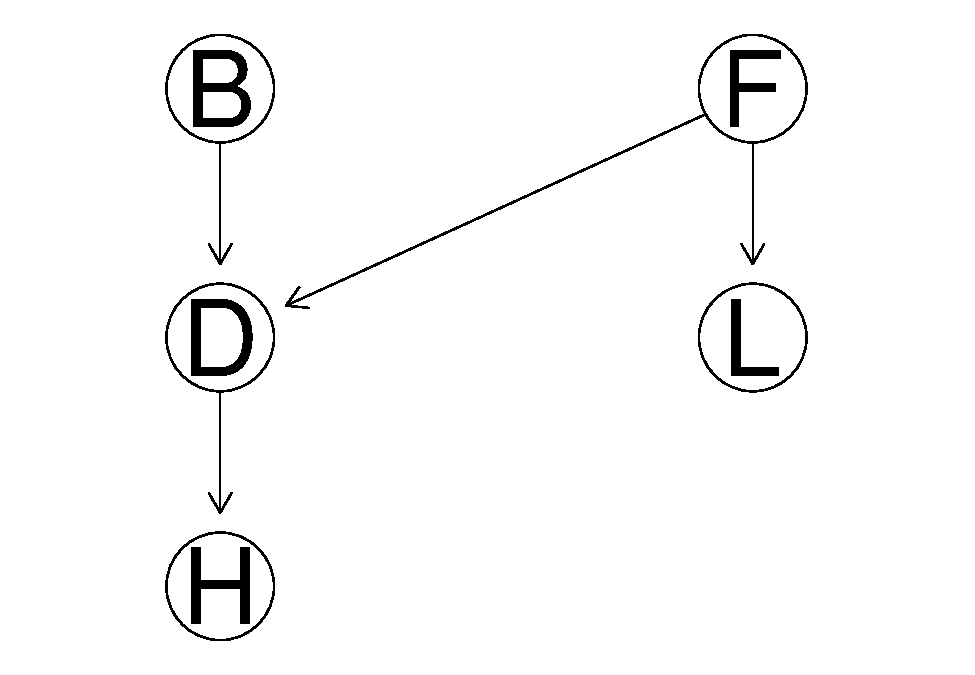
\includegraphics{FILENAME_files/figure-latex/unnamed-chunk-2-1.pdf}

Each iteration results will be collected in following arrays.

\begin{Shaded}
\begin{Highlighting}[]
\CommentTok{\#First case: P(F=TRUE) }
\NormalTok{first.mle }\OtherTok{\textless{}{-}} \FunctionTok{array}\NormalTok{(}\AttributeTok{dim =} \DecValTok{20}\NormalTok{)}
\NormalTok{first.bayes }\OtherTok{\textless{}{-}} \FunctionTok{array}\NormalTok{(}\AttributeTok{dim =} \DecValTok{20}\NormalTok{)}

\CommentTok{\#Second case: P(D=OUT | B=YES, F=TRUE)}
\NormalTok{second.mle }\OtherTok{\textless{}{-}} \FunctionTok{array}\NormalTok{(}\AttributeTok{dim =} \DecValTok{20}\NormalTok{)}
\NormalTok{second.bayes }\OtherTok{\textless{}{-}} \FunctionTok{array}\NormalTok{(}\AttributeTok{dim =} \DecValTok{20}\NormalTok{)}
\end{Highlighting}
\end{Shaded}

Now that we have a model ( fo.dag ) and data ( fo.data )
We can learn the conditional probability tables (parameters) using the bn.fit function which implements the maximum likelihood maximization and a Bayesian method to learn parameters.

\begin{Shaded}
\begin{Highlighting}[]
\ControlFlowTok{for}\NormalTok{(i }\ControlFlowTok{in} \DecValTok{1}\SpecialCharTok{:}\DecValTok{20}\NormalTok{)\{}
  \CommentTok{\#P(F=TRUE) using mle:}
\NormalTok{  first.mle[i] }\OtherTok{\textless{}{-}} \FunctionTok{bn.fit}\NormalTok{(fo.dag, fo.data[}\DecValTok{1}\SpecialCharTok{:}\NormalTok{(}\DecValTok{500}\SpecialCharTok{*}\NormalTok{i),])}\SpecialCharTok{$}\NormalTok{F}\SpecialCharTok{$}\NormalTok{prob[}\StringTok{"TRUE"}\NormalTok{]}
  \CommentTok{\#P(F=TRUE) using bayes:}
\NormalTok{  first.bayes[i] }\OtherTok{\textless{}{-}} \FunctionTok{bn.fit}\NormalTok{(fo.dag, fo.data[}\DecValTok{1}\SpecialCharTok{:}\NormalTok{(}\DecValTok{500}\SpecialCharTok{*}\NormalTok{i),], }\AttributeTok{method =} \StringTok{"bayes"}\NormalTok{, }\AttributeTok{iss=}\DecValTok{10}\NormalTok{)}\SpecialCharTok{$}\NormalTok{F}\SpecialCharTok{$}\NormalTok{prob[}\StringTok{"TRUE"}\NormalTok{]}
  
  \CommentTok{\#P(D=OUT | B=YES, F=TRUE) using mle:}
\NormalTok{  second.mle[i] }\OtherTok{\textless{}{-}} \FunctionTok{bn.fit}\NormalTok{(fo.dag, fo.data[}\DecValTok{1}\SpecialCharTok{:}\NormalTok{(}\DecValTok{500}\SpecialCharTok{*}\NormalTok{i),])}\SpecialCharTok{$}\NormalTok{D}\SpecialCharTok{$}\NormalTok{prob[}\StringTok{"OUT"}\NormalTok{,}\StringTok{"YES"}\NormalTok{,}\StringTok{"TRUE"}\NormalTok{]}
  \CommentTok{\#P(D=OUT | B=YES, F=TRUE) using bayes:}
\NormalTok{  second.bayes[i] }\OtherTok{\textless{}{-}} \FunctionTok{bn.fit}\NormalTok{(fo.dag, fo.data[}\DecValTok{1}\SpecialCharTok{:}\NormalTok{(}\DecValTok{500}\SpecialCharTok{*}\NormalTok{i),], }\AttributeTok{method =} \StringTok{"bayes"}\NormalTok{, }\AttributeTok{iss=}\DecValTok{10}\NormalTok{)}\SpecialCharTok{$}\NormalTok{D}\SpecialCharTok{$}\NormalTok{prob[}\StringTok{"OUT"}\NormalTok{,}\StringTok{"YES"}\NormalTok{,}\StringTok{"TRUE"}\NormalTok{] }
\NormalTok{\}}
\end{Highlighting}
\end{Shaded}

Plotting P(F=TRUE) using mle:

\begin{Shaded}
\begin{Highlighting}[]
\NormalTok{first.mle }\CommentTok{\#Each iteration results}
\end{Highlighting}
\end{Shaded}

\begin{verbatim}
##  [1] 0.1860000 0.1640000 0.1733333 0.1795000 0.1784000 0.1746667 0.1682857
##  [8] 0.1647500 0.1633333 0.1606000 0.1590909 0.1586667 0.1587692 0.1581429
## [15] 0.1570667 0.1561250 0.1564706 0.1560000 0.1565263 0.1566000
\end{verbatim}

\begin{Shaded}
\begin{Highlighting}[]
\NormalTok{first.mle }\OtherTok{\textless{}{-}} \FunctionTok{as.data.frame}\NormalTok{(first.mle)}
\NormalTok{first.mle}\SpecialCharTok{$}\NormalTok{ssize }\OtherTok{\textless{}{-}} \DecValTok{1}\SpecialCharTok{:}\DecValTok{20} \CommentTok{\# add iteration column}
\FunctionTok{ggplot}\NormalTok{(first.mle, }\FunctionTok{aes}\NormalTok{(ssize, first.mle)) }\SpecialCharTok{+} \FunctionTok{geom\_line}\NormalTok{() }\SpecialCharTok{+} \FunctionTok{geom\_hline}\NormalTok{(}\AttributeTok{yintercept =} \FloatTok{0.1566}\NormalTok{, }\AttributeTok{color=}\StringTok{"red"}\NormalTok{, }\AttributeTok{size=}\DecValTok{1}\NormalTok{) }\SpecialCharTok{+} \FunctionTok{xlab}\NormalTok{(}\StringTok{"iteration"}\NormalTok{) }\SpecialCharTok{+} \FunctionTok{ylab}\NormalTok{(}\StringTok{"P(F=TRUE) using MLE"}\NormalTok{) }\SpecialCharTok{+} \FunctionTok{ylim}\NormalTok{(}\FunctionTok{range}\NormalTok{(}\FloatTok{0.15}\NormalTok{,}\FloatTok{0.2}\NormalTok{))}
\end{Highlighting}
\end{Shaded}

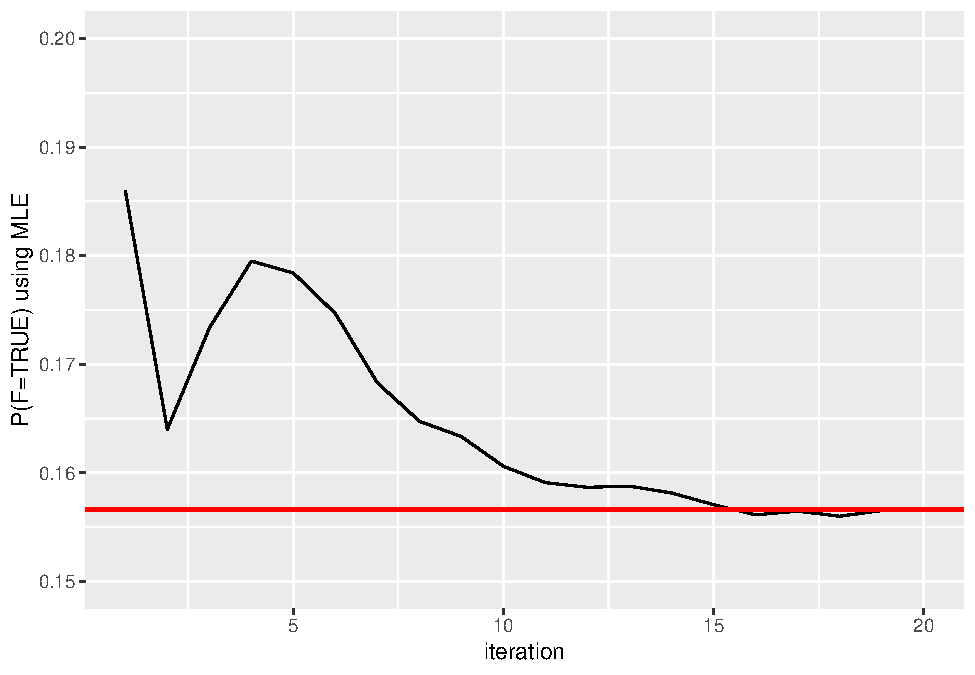
\includegraphics{FILENAME_files/figure-latex/unnamed-chunk-5-1.pdf}

Plotting P(F=TRUE) using bayes:

\begin{Shaded}
\begin{Highlighting}[]
\NormalTok{first.bayes }\CommentTok{\#Each iteration results}
\end{Highlighting}
\end{Shaded}

\begin{verbatim}
##  [1] 0.1921569 0.1673267 0.1754967 0.1810945 0.1796813 0.1757475 0.1692308
##  [8] 0.1655860 0.1640798 0.1612774 0.1597096 0.1592346 0.1592934 0.1586305
## [15] 0.1575233 0.1565543 0.1568743 0.1563818 0.1568875 0.1569431
\end{verbatim}

\begin{Shaded}
\begin{Highlighting}[]
\NormalTok{first.bayes }\OtherTok{\textless{}{-}} \FunctionTok{as.data.frame}\NormalTok{(first.bayes)}
\NormalTok{first.bayes}\SpecialCharTok{$}\NormalTok{ssize }\OtherTok{\textless{}{-}} \DecValTok{1}\SpecialCharTok{:}\DecValTok{20} \CommentTok{\# add iteration column}
\FunctionTok{ggplot}\NormalTok{(first.bayes, }\FunctionTok{aes}\NormalTok{(ssize, first.bayes)) }\SpecialCharTok{+} \FunctionTok{geom\_line}\NormalTok{() }\SpecialCharTok{+} \FunctionTok{geom\_hline}\NormalTok{(}\AttributeTok{yintercept =} \FloatTok{0.1569431}\NormalTok{, }\AttributeTok{color=}\StringTok{"red"}\NormalTok{, }\AttributeTok{size=}\DecValTok{1}\NormalTok{) }\SpecialCharTok{+} \FunctionTok{xlab}\NormalTok{(}\StringTok{"iteration"}\NormalTok{) }\SpecialCharTok{+} \FunctionTok{ylab}\NormalTok{(}\StringTok{"P(F=TRUE) using BAYES"}\NormalTok{) }\SpecialCharTok{+} \FunctionTok{ylim}\NormalTok{(}\FunctionTok{range}\NormalTok{(}\FloatTok{0.15}\NormalTok{,}\FloatTok{0.2}\NormalTok{))}
\end{Highlighting}
\end{Shaded}

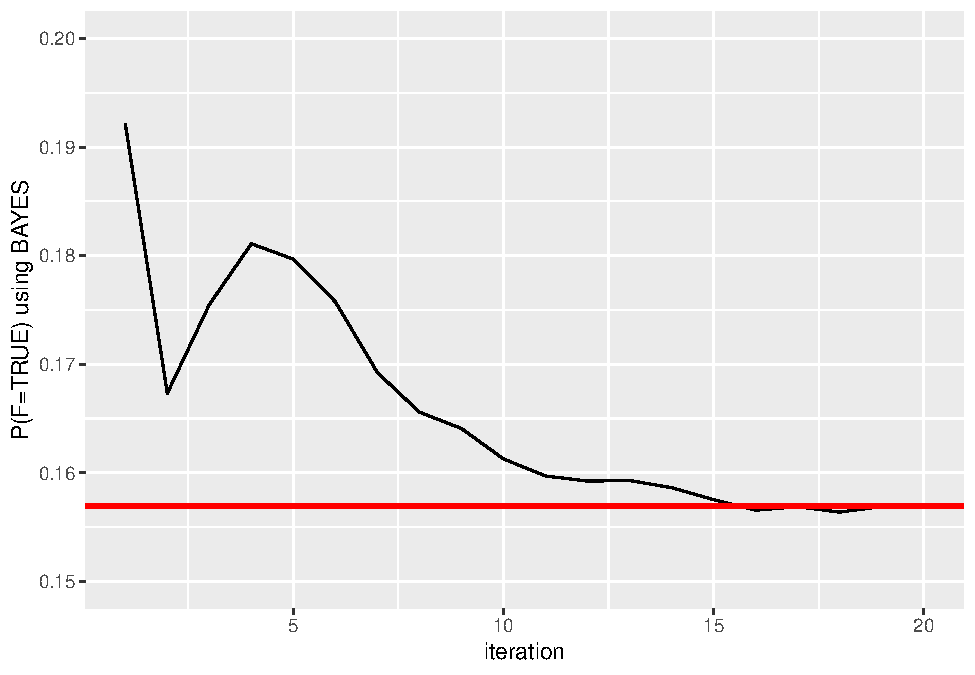
\includegraphics{FILENAME_files/figure-latex/unnamed-chunk-6-1.pdf}

Plotting P(F=TRUE) comparing both mle and bayes methods:

\begin{Shaded}
\begin{Highlighting}[]
\FunctionTok{plot}\NormalTok{(first.mle[,}\DecValTok{1}\NormalTok{], }\AttributeTok{type=}\StringTok{"l"}\NormalTok{, }\AttributeTok{col=}\StringTok{"red"}\NormalTok{, }\AttributeTok{lwd =} \DecValTok{2}\NormalTok{, }\AttributeTok{xlab=}\StringTok{"iteration"}\NormalTok{, }\AttributeTok{ylab=}\StringTok{"P(F=TRUE)"}\NormalTok{, }\AttributeTok{ylim=}\FunctionTok{range}\NormalTok{(}\FloatTok{0.15}\NormalTok{,}\FloatTok{0.20}\NormalTok{), }\AttributeTok{main=}\StringTok{"Plotting both methods"}\NormalTok{)}
\FunctionTok{lines}\NormalTok{(first.bayes[,}\DecValTok{1}\NormalTok{], }\AttributeTok{type=}\StringTok{"l"}\NormalTok{, }\AttributeTok{col=}\StringTok{"green"}\NormalTok{, }\AttributeTok{lwd =} \DecValTok{2}\NormalTok{)}
\FunctionTok{legend}\NormalTok{(}\StringTok{"topright"}\NormalTok{, }\AttributeTok{legend =} \FunctionTok{c}\NormalTok{(}\StringTok{"MLE"}\NormalTok{, }\StringTok{"BAYES"}\NormalTok{), }\AttributeTok{col =} \FunctionTok{c}\NormalTok{(}\StringTok{"red"}\NormalTok{,}\StringTok{"green"}\NormalTok{), }\AttributeTok{bty=}\StringTok{\textquotesingle{}n\textquotesingle{}}\NormalTok{, }\AttributeTok{lty=}\DecValTok{1}\NormalTok{, }\AttributeTok{lwd=}\DecValTok{2}\NormalTok{)}
\end{Highlighting}
\end{Shaded}

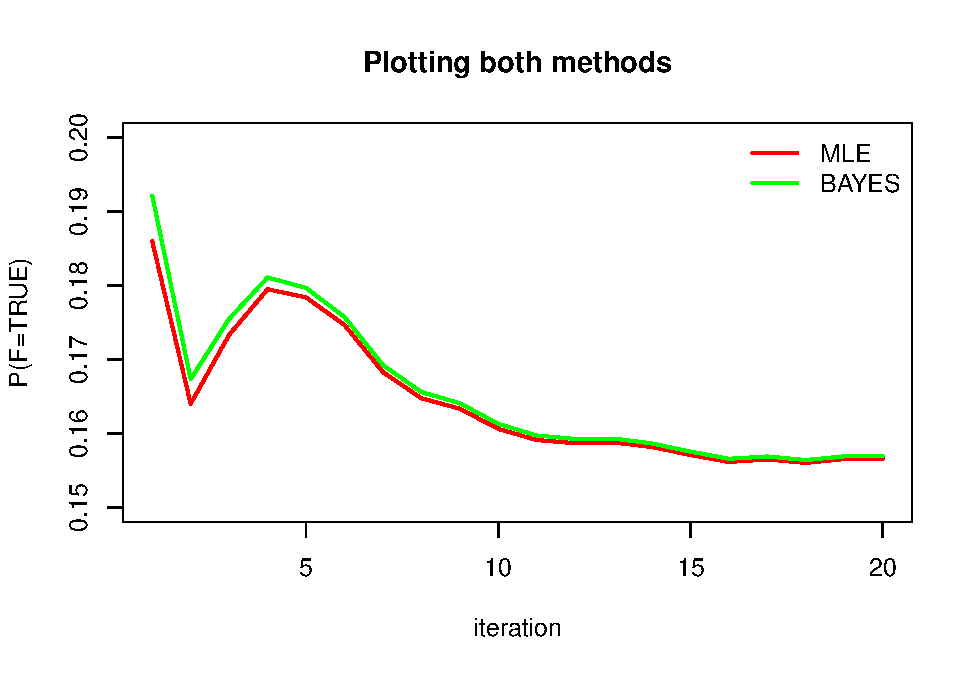
\includegraphics{FILENAME_files/figure-latex/unnamed-chunk-7-1.pdf}

Plotting P(D=OUT \textbar{} B=YES, F=TRUE) using mle:

\begin{Shaded}
\begin{Highlighting}[]
\NormalTok{second.mle }\CommentTok{\#Each iteration results}
\end{Highlighting}
\end{Shaded}

\begin{verbatim}
##  [1] 1 1 1 1 1 1 1 1 1 1 1 1 1 1 1 1 1 1 1 1
\end{verbatim}

\begin{Shaded}
\begin{Highlighting}[]
\NormalTok{second.mle }\OtherTok{\textless{}{-}} \FunctionTok{as.data.frame}\NormalTok{(second.mle)}
\NormalTok{second.mle}\SpecialCharTok{$}\NormalTok{ssize }\OtherTok{\textless{}{-}} \DecValTok{1}\SpecialCharTok{:}\DecValTok{20} \CommentTok{\# add iteration column}
\FunctionTok{ggplot}\NormalTok{(second.mle, }\FunctionTok{aes}\NormalTok{(ssize, second.mle)) }\SpecialCharTok{+} \FunctionTok{geom\_line}\NormalTok{() }\SpecialCharTok{+} \FunctionTok{geom\_hline}\NormalTok{(}\AttributeTok{yintercept =} \DecValTok{1}\NormalTok{, }\AttributeTok{color=}\StringTok{"red"}\NormalTok{, }\AttributeTok{size=}\DecValTok{1}\NormalTok{) }\SpecialCharTok{+} \FunctionTok{xlab}\NormalTok{(}\StringTok{"iteration"}\NormalTok{) }\SpecialCharTok{+} \FunctionTok{ylab}\NormalTok{(}\StringTok{"P(D=OUT | B=YES, F=TRUE) using MLE"}\NormalTok{) }\SpecialCharTok{+} \FunctionTok{ylim}\NormalTok{(}\FunctionTok{range}\NormalTok{(}\DecValTok{0}\NormalTok{,}\DecValTok{1}\NormalTok{))}
\end{Highlighting}
\end{Shaded}

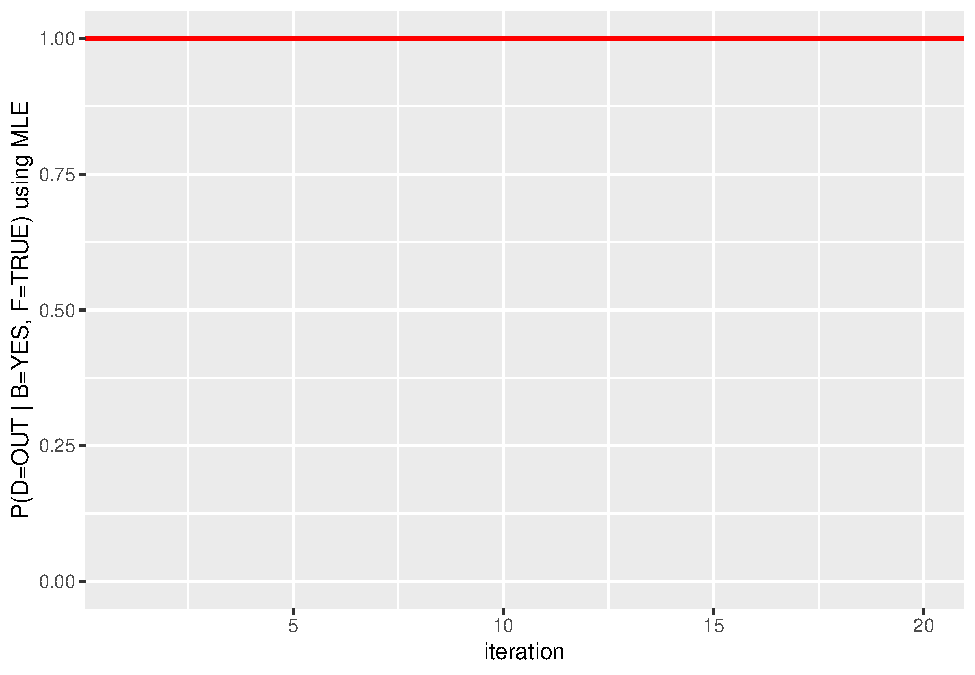
\includegraphics{FILENAME_files/figure-latex/unnamed-chunk-8-1.pdf}

Plotting P(D=OUT \textbar{} B=YES, F=TRUE) using bayes:

\begin{Shaded}
\begin{Highlighting}[]
\NormalTok{second.bayes }\CommentTok{\#Each iteration results}
\end{Highlighting}
\end{Shaded}

\begin{verbatim}
##  [1] 0.6428571 0.6428571 0.6428571 0.7222222 0.7727273 0.7727273 0.7727273
##  [8] 0.8076923 0.8333333 0.8529412 0.8529412 0.8809524 0.8809524 0.9000000
## [15] 0.9000000 0.9074074 0.9193548 0.9242424 0.9324324 0.9324324
\end{verbatim}

\begin{Shaded}
\begin{Highlighting}[]
\NormalTok{second.bayes }\OtherTok{\textless{}{-}} \FunctionTok{as.data.frame}\NormalTok{(second.bayes)}
\NormalTok{second.bayes}\SpecialCharTok{$}\NormalTok{ssize }\OtherTok{\textless{}{-}} \DecValTok{1}\SpecialCharTok{:}\DecValTok{20} \CommentTok{\# add iteration column}
\FunctionTok{ggplot}\NormalTok{(second.bayes, }\FunctionTok{aes}\NormalTok{(ssize, second.bayes)) }\SpecialCharTok{+} \FunctionTok{geom\_line}\NormalTok{() }\SpecialCharTok{+} \FunctionTok{geom\_hline}\NormalTok{(}\AttributeTok{yintercept =} \FloatTok{0.9324324}\NormalTok{, }\AttributeTok{color=}\StringTok{"red"}\NormalTok{, }\AttributeTok{size=}\DecValTok{1}\NormalTok{) }\SpecialCharTok{+} \FunctionTok{xlab}\NormalTok{(}\StringTok{"iteration"}\NormalTok{) }\SpecialCharTok{+} \FunctionTok{ylab}\NormalTok{(}\StringTok{"P(D=OUT | B=YES, F=TRUE) using BAYES"}\NormalTok{) }\SpecialCharTok{+} \FunctionTok{ylim}\NormalTok{(}\FunctionTok{range}\NormalTok{(}\DecValTok{0}\NormalTok{,}\DecValTok{1}\NormalTok{))}
\end{Highlighting}
\end{Shaded}

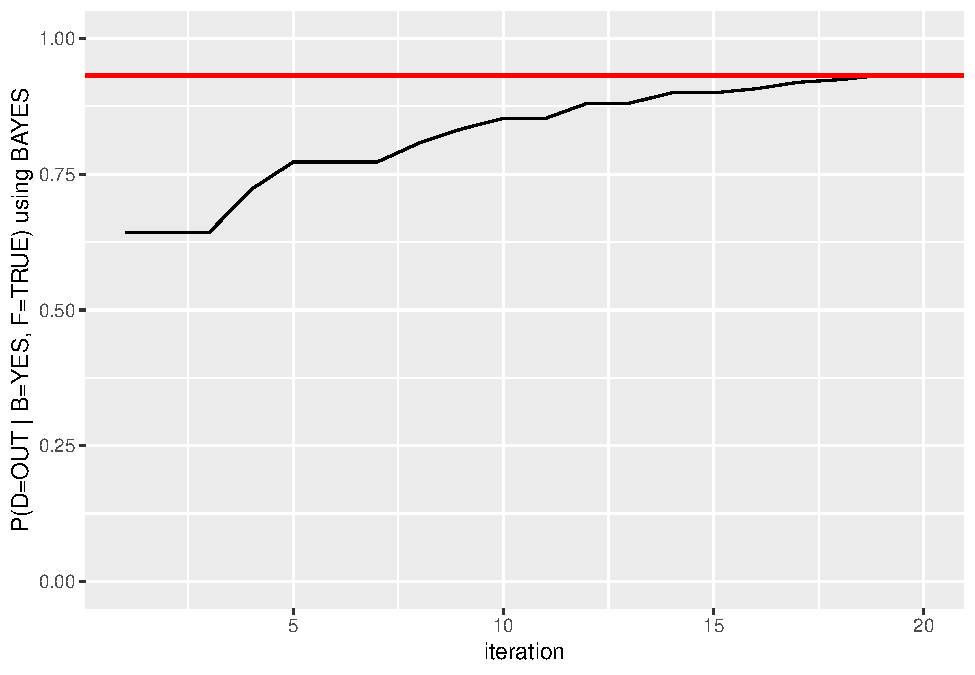
\includegraphics{FILENAME_files/figure-latex/unnamed-chunk-9-1.pdf}

Plotting P(D=OUT \textbar{} B=YES, F=TRUE) comparing both mle and bayes methods:

\begin{Shaded}
\begin{Highlighting}[]
\FunctionTok{plot}\NormalTok{(second.mle[,}\DecValTok{1}\NormalTok{], }\AttributeTok{type=}\StringTok{"l"}\NormalTok{, }\AttributeTok{col=}\StringTok{"red"}\NormalTok{, }\AttributeTok{lwd =} \DecValTok{2}\NormalTok{, }\AttributeTok{xlab=}\StringTok{"iteration"}\NormalTok{, }\AttributeTok{ylab=}\StringTok{"P(D=OUT | B=YES, F=TRUE)"}\NormalTok{, }\AttributeTok{ylim=}\FunctionTok{range}\NormalTok{(}\FloatTok{0.6}\NormalTok{,}\DecValTok{1}\NormalTok{), }\AttributeTok{main=}\StringTok{"Plotting both methods"}\NormalTok{)}
\FunctionTok{lines}\NormalTok{(second.bayes[,}\DecValTok{1}\NormalTok{], }\AttributeTok{type=}\StringTok{"l"}\NormalTok{, }\AttributeTok{col=}\StringTok{"green"}\NormalTok{, }\AttributeTok{lwd =} \DecValTok{2}\NormalTok{)}
\FunctionTok{legend}\NormalTok{(}\StringTok{"bottomright"}\NormalTok{, }\AttributeTok{legend =} \FunctionTok{c}\NormalTok{(}\StringTok{"MLE"}\NormalTok{, }\StringTok{"BAYES"}\NormalTok{), }\AttributeTok{col =} \FunctionTok{c}\NormalTok{(}\StringTok{"red"}\NormalTok{,}\StringTok{"green"}\NormalTok{), }\AttributeTok{bty=}\StringTok{\textquotesingle{}n\textquotesingle{}}\NormalTok{, }\AttributeTok{lty=}\DecValTok{1}\NormalTok{, }\AttributeTok{lwd=}\DecValTok{2}\NormalTok{)}
\end{Highlighting}
\end{Shaded}

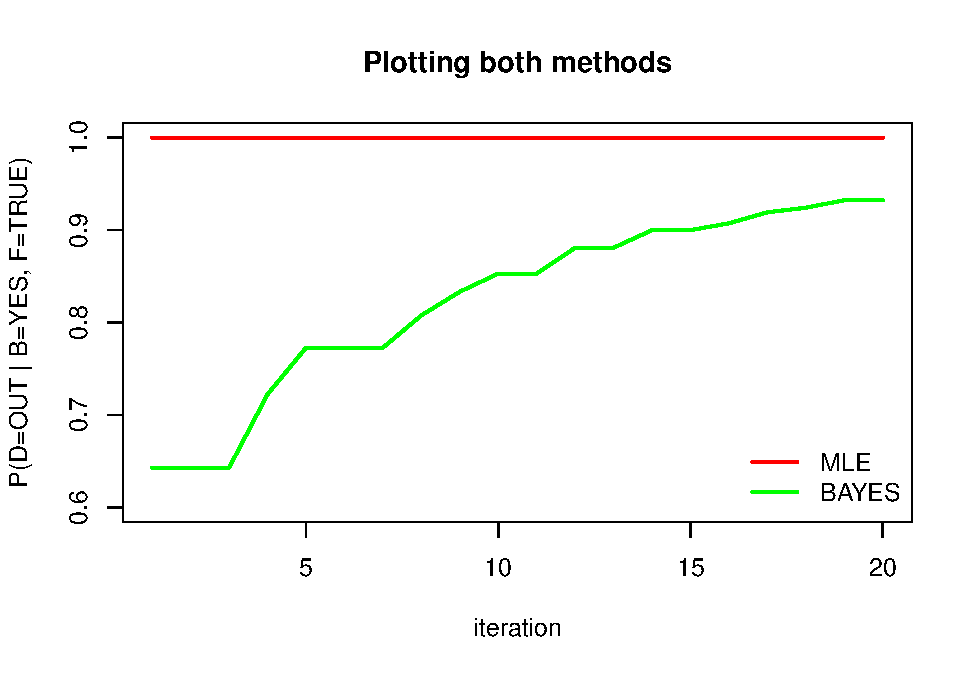
\includegraphics{FILENAME_files/figure-latex/unnamed-chunk-10-1.pdf}

\hypertarget{references}{%
\section*{References}\label{references}}
\addcontentsline{toc}{section}{References}

\hypertarget{appendices}{%
\section*{Appendices}\label{appendices}}
\addcontentsline{toc}{section}{Appendices}

\hypertarget{about-author}{%
\subsection*{About Author}\label{about-author}}
\addcontentsline{toc}{subsection}{About Author}

\end{document}
